\documentclass[
  12pt,
  oneside,
  a4paper,
  article,
  brazil
]{USPSC-classe/USPSC}

\usepackage[T1]{fontenc}
\usepackage[utf8]{inputenc}
\usepackage{lmodern}
\usepackage{microtype}
\usepackage{indentfirst}
\usepackage{graphicx}
\usepackage{booktabs}
\usepackage{array}
\usepackage{tabularx}
\usepackage{amsmath,amssymb}
\usepackage[section]{placeins}

\hypersetup{
  pdftitle={Estudo de disciplinas ICMC-USP},
  pdfauthor={Gabriel Carbinatto, Enzo Castelo Branco Biondi e Matheus Rodrigues Ferreira},
  pdfsubject={SCC5836 Visualização Computacional},
  pdfkeywords={visualização computacional, disciplinas, currículo, requisitos, tópicos, ICMC},
  colorlinks=true,
  linkcolor=black,
  citecolor=black,
  urlcolor=black
}

\setlrmarginsandblock{3cm}{2cm}{*}
\setulmarginsandblock{3cm}{2cm}{*}
\checkandfixthelayout
\setlength{\parindent}{1.3cm}
\setlength{\parskip}{0.2cm}

\renewcommand{\ABNTEXsectionfontsize}{\fontsize{12}{14}\bfseries}
\renewcommand{\ABNTEXsubsectionfontsize}{\fontsize{12}{14}\bfseries}
\renewcommand{\ABNTEXsubsubsectionfontsize}{\fontsize{12}{14}\normalfont}
\renewcommand{\ABNTEXcaptiondelim}{:~}
\captiondelim{:~}
\setlength{\cftlastnumwidth}{2.2em}
\cftsetindents{section}{0em}{\cftlastnumwidth}
\cftsetindents{subsection}{0em}{\cftlastnumwidth}

\begin{document}
\selectlanguage{brazil}
\frenchspacing

\hypersetup{pageanchor=false}
\begin{titlingpage}
  \begin{center}
    {\large Universidade de São Paulo\par}
    \vspace{0.15cm}
    {\large Instituto de Ciências Matemáticas e de Computação\par}

    \vspace*{3.3cm}

    {\Large\bfseries Estudo de disciplinas ICMC-USP\par}

    \vspace{0.8cm}

    {\large SCC5836 Visualização Computacional\par}

    \vfill

    {\large\bfseries Gabriel Carbinatto\par}
    {\normalsize Número USP: 12725411\par}

    \vspace{0.45cm}

    {\large\bfseries Enzo Castelo Branco Biondi\par}
    {\normalsize Número USP: 14568142\par}

    \vspace{0.45cm}

    {\large\bfseries Matheus Rodrigues Ferreira\par}
    {\normalsize Número USP: 14762149\par}

    \vfill

    {\normalsize São Carlos\par}
    {\normalsize 26 de novembro de 2026\par}
  \end{center}
\end{titlingpage}
\hypersetup{pageanchor=true}
\setcounter{page}{2}

\pdfbookmark[0]{\contentsname}{toc}
\tableofcontents*
\thispagestyle{empty}
\clearpage
\pagestyle{simple}

\section{Introdução}

As grades de graduação do Instituto de Ciências Matemáticas e de Computação
(ICMC-USP) reúnem disciplinas de computação, matemática, estatística e áreas
relacionadas. A consulta a essas grades pelo JúpiterWeb é adequada para localizar
uma disciplina ou acompanhar um curso específico, mas não oferece uma visão
conjunta do conteúdo das ementas, das relações de requisito e da distribuição da
carga horária entre assuntos. Como consequência, perguntas e análises
comparativas exigem percorrer várias páginas de maneira manual.

Este projeto organiza essas informações em um conjunto de dados único e propõe
uma exploração visual das disciplinas do ICMC. A primeira entrega documentou a
criação e o processamento desse conjunto e avaliou três visualizações
interativas para reconhecer agrupamentos temáticos, comparar a similaridade
entre ementas e examinar encadeamentos curriculares. A segunda entrega
acrescenta nuvens de palavras, uma composição da carga horária por tópico e
mecanismos de seleção coordenada e consulta dinâmica. O sistema foi
implementado como uma página em D3, publicada no GitHub Pages.

\subsection{Coleta dos dados}

Os cursos foram selecionados a partir do site do ICMC, e suas 12 grades
curriculares foram consultadas no JúpiterWeb. Para cada código encontrado nas
grades, são consultadas as páginas da disciplina e de seus requisitos.
As respostas HTML são mantidas em cache para que a extração possa ser
reproduzida sem repetir as consultas ao sistema.

As grades reúnem 1.089 registros curriculares, correspondentes a 582 códigos
distintos. O percurso pelas relações de requisito acrescenta 54 códigos que não
aparecem diretamente nas grades. Ao final, foram coletadas 636 disciplinas. A
Tabela~\ref{tab:cobertura} resume essa cobertura.

\begin{table}[htbp]
  \centering
  \caption{Disciplinas coletadas no JúpiterWeb.}
  \label{tab:cobertura}
  \begin{tabularx}{\linewidth}{>{\raggedright\arraybackslash}X r}
    \toprule
    \textbf{Origem} & \textbf{Disciplinas} \\
    \midrule
    Disciplinas presentes nas grades & 582 \\
    Disciplinas adicionadas pelas relações de requisito & 54 \\
    \textbf{Total coletado} & \textbf{636} \\
    \bottomrule
  \end{tabularx}
\end{table}

Cada disciplina coletada contém identificação, departamento, créditos, carga
horária, ementa, objetivos, conteúdo programático e docentes. As grades e as
relações de requisito são armazenadas em tabelas separadas e vinculadas pelos
códigos das disciplinas. As variáveis são de quatro tipos: textuais (ementa,
objetivos e conteúdo programático), categóricas (departamento, curso e tipo de
disciplina), numéricas (créditos, carga horária e semestre ideal) e relacionais
(requisitos entre disciplinas).

\newpage  

\subsection{Perguntas de pesquisa}

A análise foi organizada em torno de três questões:

\begin{enumerate}
  \item Como as disciplinas se agrupam a partir de suas ementas?
  \item Quais disciplinas são mais semelhantes a uma disciplina de interesse?
  \item Como a grade de cada curso organiza as disciplinas por requisitos e
  distribui sua carga horária entre os tópicos?
\end{enumerate}

A primeira questão trata da estrutura global das ementas das disciplinas. A
segunda torna explícitos os valores de similaridade em torno de uma disciplina.
A terceira trata dos requisitos e da distribuição da carga horária por tópico
em cada curso.

\section{Metodologia}

A metodologia converte os registros coletados em disciplinas únicas, representa
seus textos em um espaço vetorial comum e deriva desse espaço as medidas de
agrupamento e similaridade.

\subsection{Tratamento dos dados}

Os campos textuais são normalizados em Unicode NFC e têm espaços repetidos
removidos. Em seguida, ementa, objetivos e conteúdo programático são
concatenados para cada código. Como mostra a Tabela~\ref{tab:textos}, essa
combinação preserva 11 dos 15 registros sem ementa, que ainda contêm objetivos
ou conteúdo programático. Os quatro registros sem texto ficam abaixo do mínimo
de 80 caracteres e são excluídos, restando 632 códigos para análise.

\begin{table}[htbp]
  \centering
  \caption{Disponibilidade dos campos textuais nos 636 registros coletados.}
  \label{tab:textos}
  \begin{tabularx}{\linewidth}{>{\raggedright\arraybackslash}X r}
    \toprule
    \textbf{Campo} & \textbf{Registros com texto} \\
    \midrule
    Ementa & 621 \\
    Objetivos & 632 \\
    Conteúdo programático & 632 \\
    Pelo menos um dos três campos & 632 \\
    \bottomrule
  \end{tabularx}
\end{table}

Nome, departamento, carga horária e requisitos não compõem o texto representado
nem as medidas de agrupamento e similaridade. Esses atributos permanecem
associados aos registros para identificação, filtragem e interpretação dos
resultados.

\subsection{Disciplinas únicas}

Um mesmo conteúdo pode estar cadastrado sob códigos diferentes, como as versões
presencial e semipresencial de Cálculo I. Para que essas cópias não sejam
contadas mais de uma vez, os códigos são reunidos em disciplinas únicas. Seja
$s_{\mathrm{tf}}(a,b)$ o cosseno entre os vetores TF-IDF dos textos dos códigos
$a$ e $b$. Os dois códigos são reunidos quando

\begin{equation}
  \bigl[\,n(a)=n(b)\ \wedge\ s_{\mathrm{tf}}(a,b)\geq\tau_{\mathrm{nome}}\,\bigr]
  \ \vee\
  \bigl[\,\nu(a)=\nu(b)\ \wedge\ s_{\mathrm{tf}}(a,b)\geq0{,}90\,\bigr],
  \label{eq:duplicidade}
\end{equation}

em que $n(a)$ é o nome normalizado e $\nu(a)$, a numeração (I, II, III). O nome
atua apenas como identificador do registro: ele propõe candidatos, e a fusão
exige confirmação pelo texto. O limiar $\tau_{\mathrm{nome}}=0{,}099$ é o
percentil 99 de $s_{\mathrm{tf}}$ entre todos os pares. Assim, homônimas de
conteúdos distintos, como Física III do IFSC e Física 3 da Licenciatura em
Ciências Exatas, permanecem separadas. A condição sobre a numeração impede a
fusão de disciplinas sequenciais com textos quase idênticos.

Os pares aceitos são fechados transitivamente por união-busca, o que reduz 632
códigos com texto a 528 disciplinas únicas. O texto de cada disciplina única
reúne os textos distintos de seus códigos, e os requisitos são reescritos com os
novos identificadores.

\subsection{Representação textual}

Os textos são representados pelo modelo multilíngue BGE-M3 \cite{chen2024},
que produz vetores de 1.024 dimensões e lê até 8.192 tokens por entrada. Como o
maior texto do conjunto tem 1.523 tokens, cada disciplina é codificada
integralmente em uma única entrada, sem divisão em blocos.

Seja $f(x_d)$ a saída do modelo para o texto $x_d$ da disciplina $d$. O vetor da
disciplina e a similaridade entre as disciplinas $a$ e $b$ são

\begin{equation}
  \boldsymbol{e}_d=\frac{f(x_d)}{\lVert f(x_d)\rVert_2},
  \qquad
  s(a,b)=\boldsymbol{e}_a^{\mathsf T}\boldsymbol{e}_b.
  \label{eq:embedding}
\end{equation}

Entre os 139.128 pares de disciplinas, a mediana de $s$ é 0,54. Como a escala do
cosseno depende do modelo, os limiares usados nas visualizações são percentis
dessa distribuição, e não valores fixos.

\subsection{Agrupamento temático}

Os tópicos são obtidos com BERTopic \cite{grootendorst2022}, aplicado aos
embeddings de~\eqref{eq:embedding} e aos textos das disciplinas. O UMAP
\cite{mcinnes2018} reduz os vetores a cinco dimensões, e o HDBSCAN
\cite{mcinnes2017} identifica grupos com pelo menos oito disciplinas. Foram
encontrados 24 tópicos. As 74 disciplinas classificadas como ruído recebem o
tópico de centroide mais próximo no espaço de 1.024 dimensões.

Cada tópico é descrito pelos termos que o distinguem dos demais, segundo o
c-TF-IDF. O peso do termo $t$ no tópico $c$ é

\begin{equation}
  w_{t,c}=\operatorname{tf}_{t,c}
  \log\!\left(1+\frac{A}{f_t}\right),
  \label{eq:ctfidf}
\end{equation}

em que $\operatorname{tf}_{t,c}$ é a frequência relativa de $t$ no conjunto dos
textos de $c$, $f_t$ é a frequência de $t$ em todos os tópicos e $A$ é o número
médio de palavras por tópico. O peso cresce com a presença do termo no tópico e
diminui com sua presença no restante do conjunto. Palavras funcionais e termos
genéricos de ementa, como ``disciplina'' e ``objetivo'', são excluídos antes do
cálculo. Os nomes dos
tópicos foram atribuídos após a inspeção dos termos de maior peso e das
disciplinas de cada grupo. Eles resumem o conteúdo e não são produzidos pelo
modelo.

\newpage

\section{Visualizações interativas}

O sistema é uma página web construída com D3 \cite{bostock2011} e reúne cinco
visualizações: um mapa de agrupamentos, nuvens de palavras por tópico, uma
comparação de similaridade a partir de uma disciplina de referência, a grade
curricular com seus requisitos e um treemap da composição de cada curso. As
cinco compartilham uma paleta de 24 cores, uma por tópico,
ordenada para que tópicos próximos recebam matizes vizinhos, de modo que cada
disciplina mantém a mesma cor em todas as visões.

O projeto visual tomou como referência, de maneira geral, trabalhos de
visualização e design da informação de Cédric Scherer e de Yan Holtz, como a
página D3 Graph Gallery \cite{scherer,holtz}.

\subsection{Mapa de agrupamentos}

Como a similaridade define relações entre pares de disciplinas, a primeira
questão é representada por uma rede sobre uma projeção bidimensional, que mostra
ao mesmo tempo os grupos e as vizinhanças. A Figura~\ref{fig:mapa} representa disciplinas por pontos e tópicos por cores.
As posições resultam de uma segunda execução do UMAP, em duas dimensões,
independente da redução usada no agrupamento. As coordenadas são giradas para
que o eixo de maior variância fique na horizontal e reescaladas por um único
fator, preservando as proporções da projeção. Textos idênticos são projetados
uma única vez e compartilham a coordenada, pois, caso contrário, o UMAP os
isolaria como componente desconexo. Para evitar sobreposição, cada ponto é
afastado de seus vizinhos por uma repulsão de colisão, presa à posição original.
O deslocamento mediano é de 1 pixel e o máximo, de 12 pixels, em um mapa de
1.234 pixels de largura.

As linhas ligam disciplinas semelhantes. Seja $\mathcal{N}_4(a)$ o conjunto das
quatro disciplinas mais semelhantes a $a$ e $\operatorname{nn}(a)$ a mais
semelhante. As arestas são

\begin{equation}
  \mathcal{E}=\bigl\{\{a,b\}: b\in\mathcal{N}_4(a),\ s(a,b)\geq\tau_{\mathrm{rede}}\bigr\}
  \cup\bigl\{\{a,\operatorname{nn}(a)\}\bigr\},
  \label{eq:arestas}
\end{equation}

em que $\tau_{\mathrm{rede}}=0{,}603$ é o percentil 85 de $s$. A segunda parcela
impede pontos isolados, e a rede resultante possui 1.499 arestas.

Ao selecionar uma disciplina, suas cinco vizinhas mais semelhantes recebem
números no mapa, repetidos com seus nomes em um índice abaixo dele, e as demais
são esmaecidas. O mapa favorece a leitura de vizinhanças, mas não é uma escala
métrica: o UMAP preserva sobretudo relações locais, e distâncias visuais iguais
podem corresponder a similaridades diferentes. Por isso, os valores informados
ao usuário são sempre calculados nos embeddings.

\begin{figure}[htbp]
  \centering
  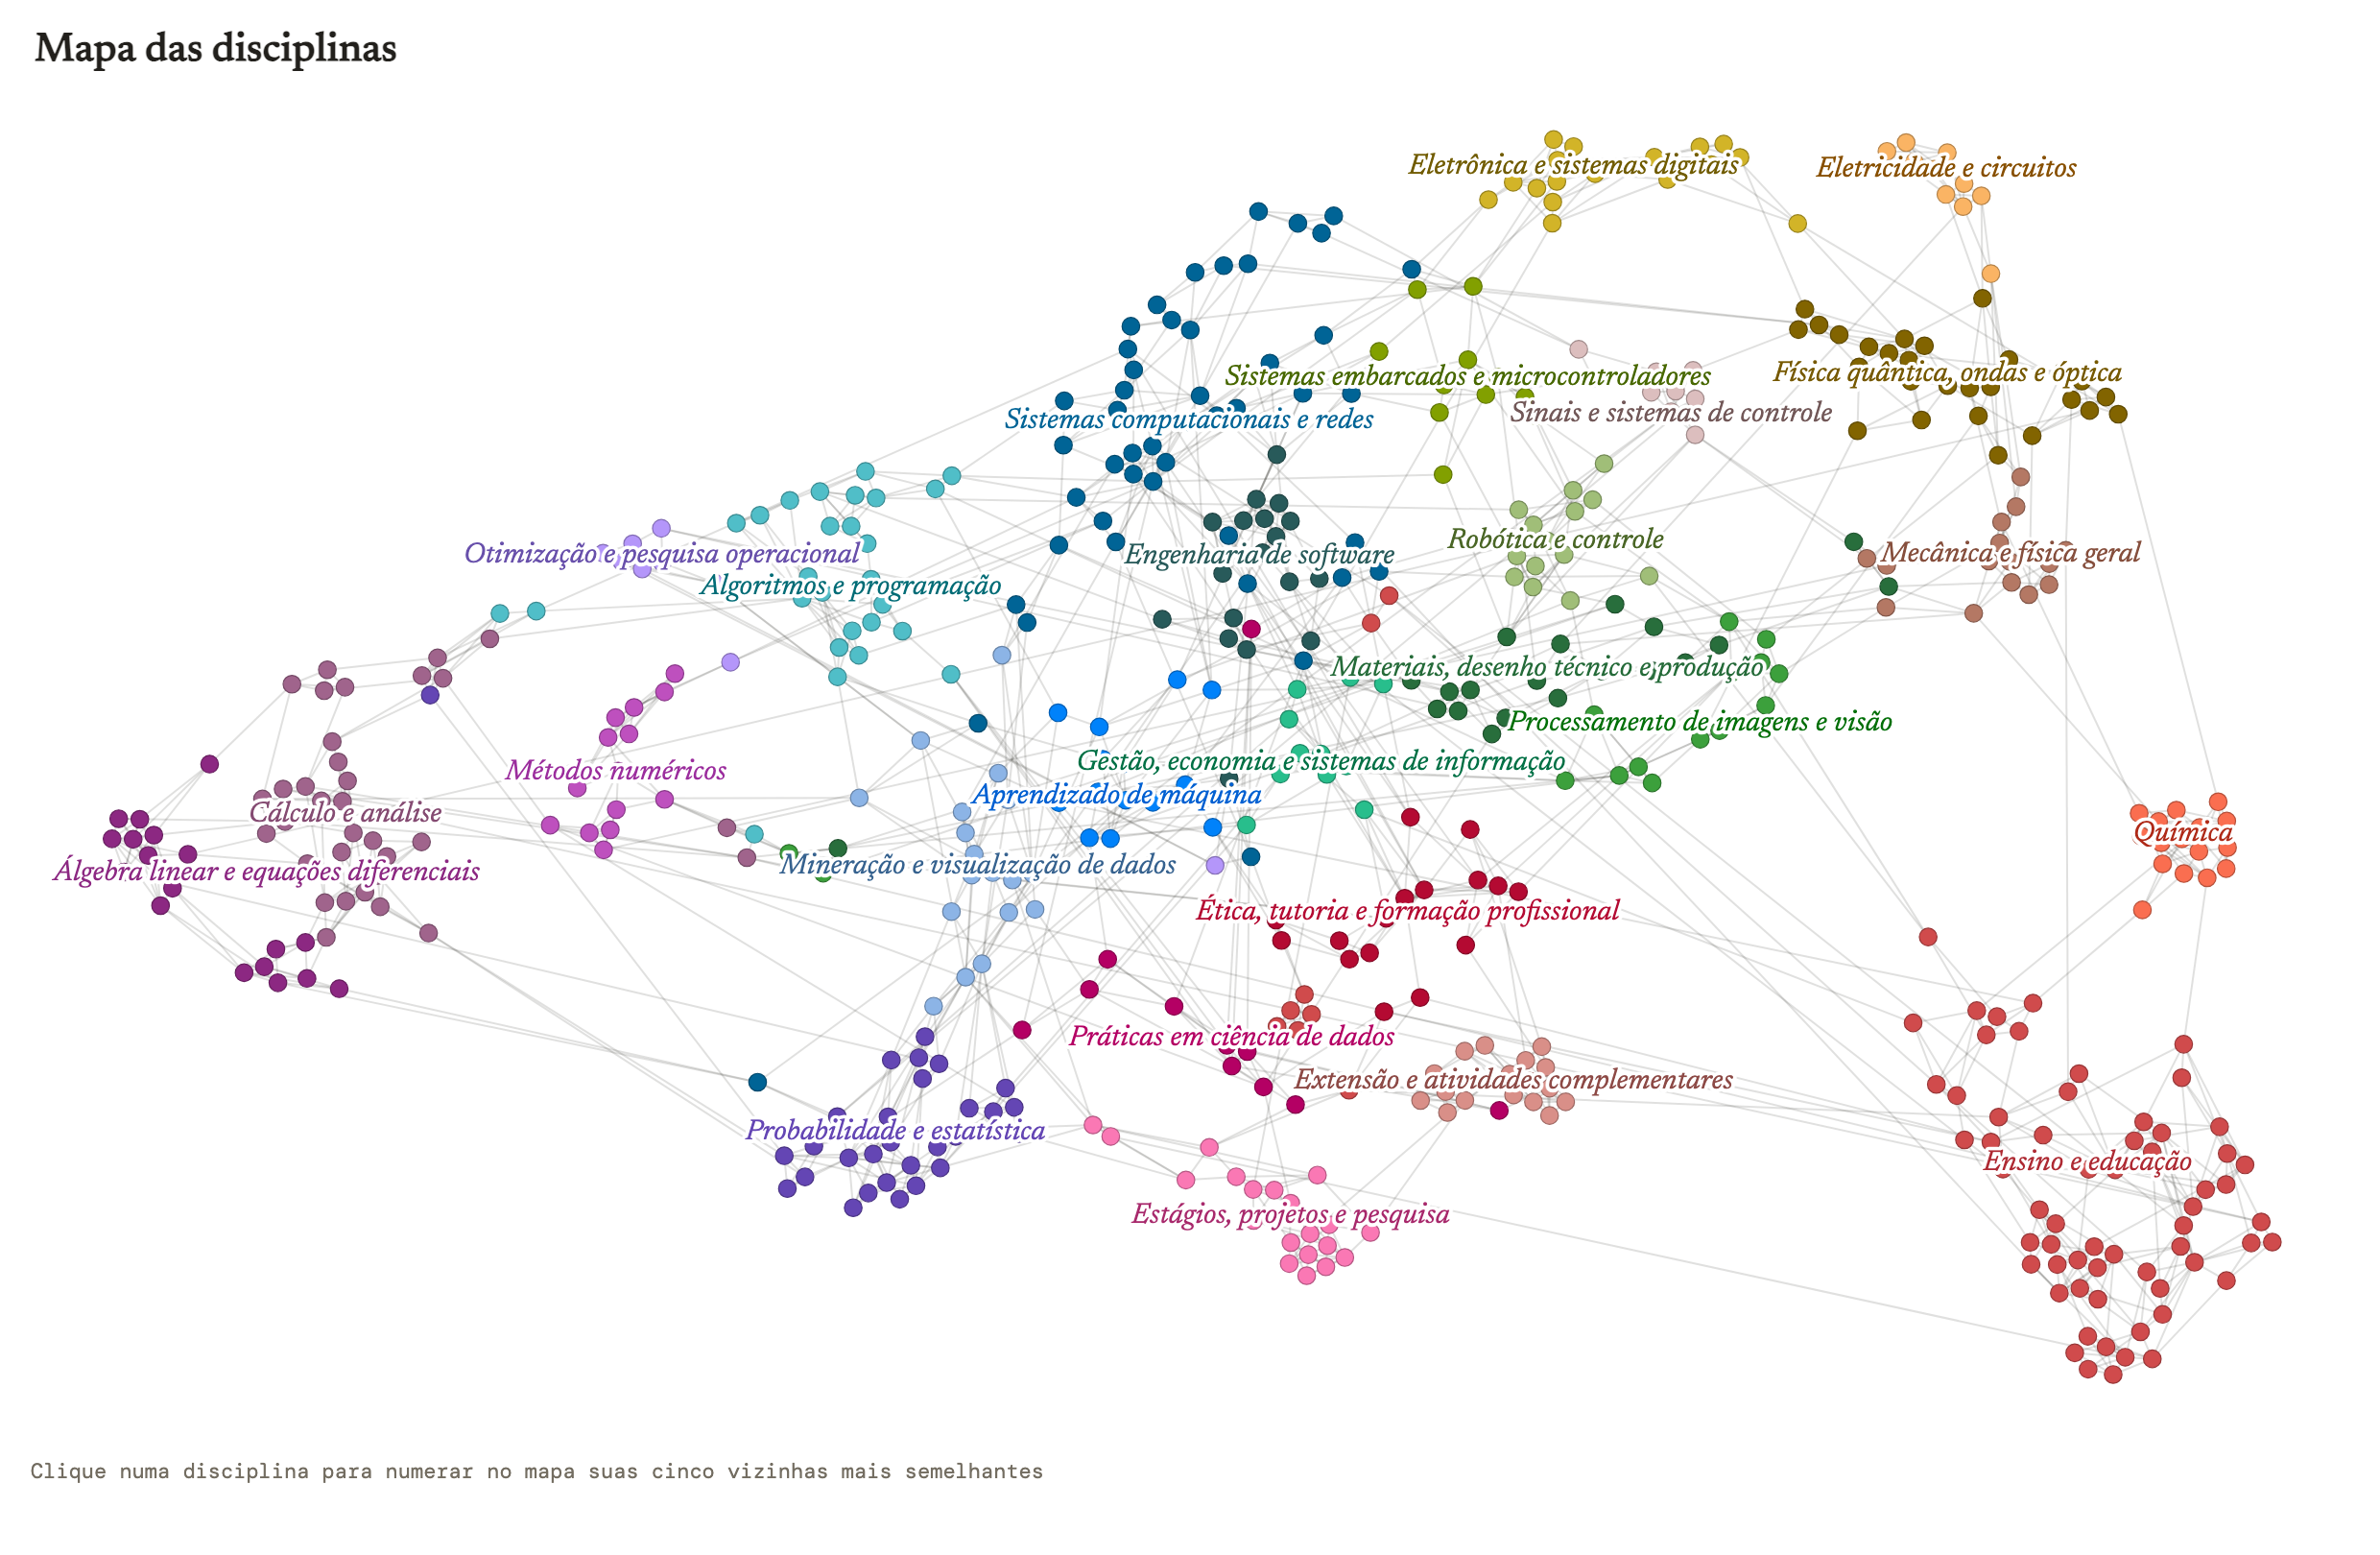
\includegraphics[width=\linewidth]{figures/mapa.png}
  \caption{Mapa das 528 disciplinas únicas em seu estado inicial. As cores
  indicam os 24 tópicos e as linhas representam relações de vizinhança textual.}
  \label{fig:mapa}
\end{figure}

\subsection{Palavras de cada tópico}

As nuvens de palavras partem dos 24 termos de maior peso c-TF-IDF em cada
tópico, segundo~\eqref{eq:ctfidf}. O tamanho representa o peso dentro da nuvem;
por isso, palavras maiores são mais características daquele tópico, mas os
tamanhos não devem ser comparados diretamente entre nuvens. A
Figura~\ref{fig:nuvens} mostra quatro exemplos. A seleção de uma nuvem destaca
no mapa as disciplinas do tópico correspondente; uma segunda seleção remove o
filtro. A mesma seleção pode ser feita pelo rótulo do tópico no treemap.

\begin{figure}[htbp]
  \centering
  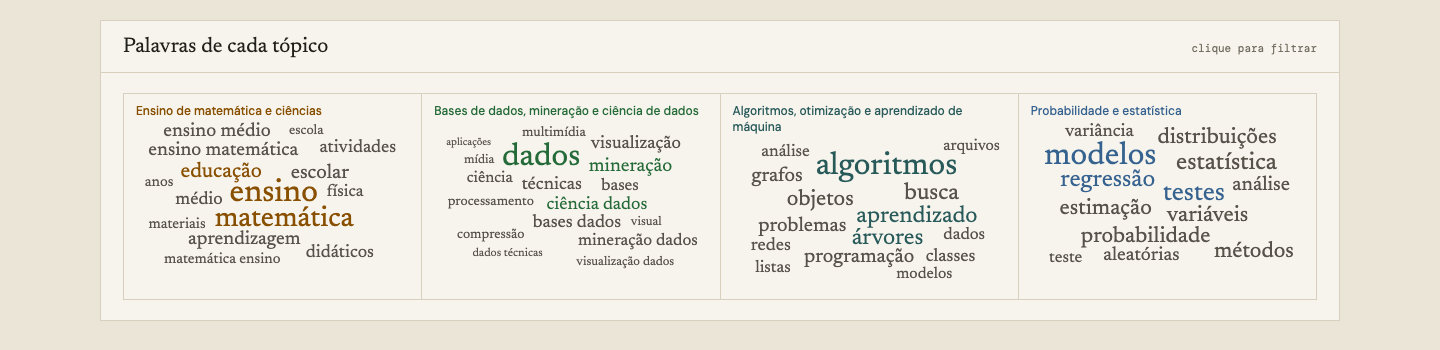
\includegraphics[width=\linewidth]{figures/nuvens.png}
  \caption{Nuvens de palavras de quatro tópicos. A dimensão dos termos
  representa seus pesos c-TF-IDF em cada tópico.}
  \label{fig:nuvens}
\end{figure}

\newpage

\subsection{Similaridade entre disciplinas}

A Figura~\ref{fig:similaridade} mostra, para uma referência escolhida pelo
usuário, as disciplinas acima do limiar de similaridade, inicialmente 0,619, o
percentil 90 de $s$, uma linha por tópico. A posição horizontal é a
similaridade $s$, e o
deslocamento vertical apenas evita a sobreposição. As linhas são ordenadas pela
maior similaridade de cada tópico, e as cinco disciplinas mais próximas recebem
numeração e um índice textual, sendo exibidas mesmo abaixo do limiar. Em
relação ao mapa, o \emph{beeswarm} explicita a magnitude da similaridade e
permite comparar tópicos em uma escala comum. Um controle deslizante permite
alterar o limiar entre 0,500 e 0,850 e atualiza imediatamente as disciplinas
exibidas. As cinco mais próximas permanecem visíveis mesmo abaixo do limite,
para preservar a comparação local.

\begin{figure}[htbp]
  \centering
  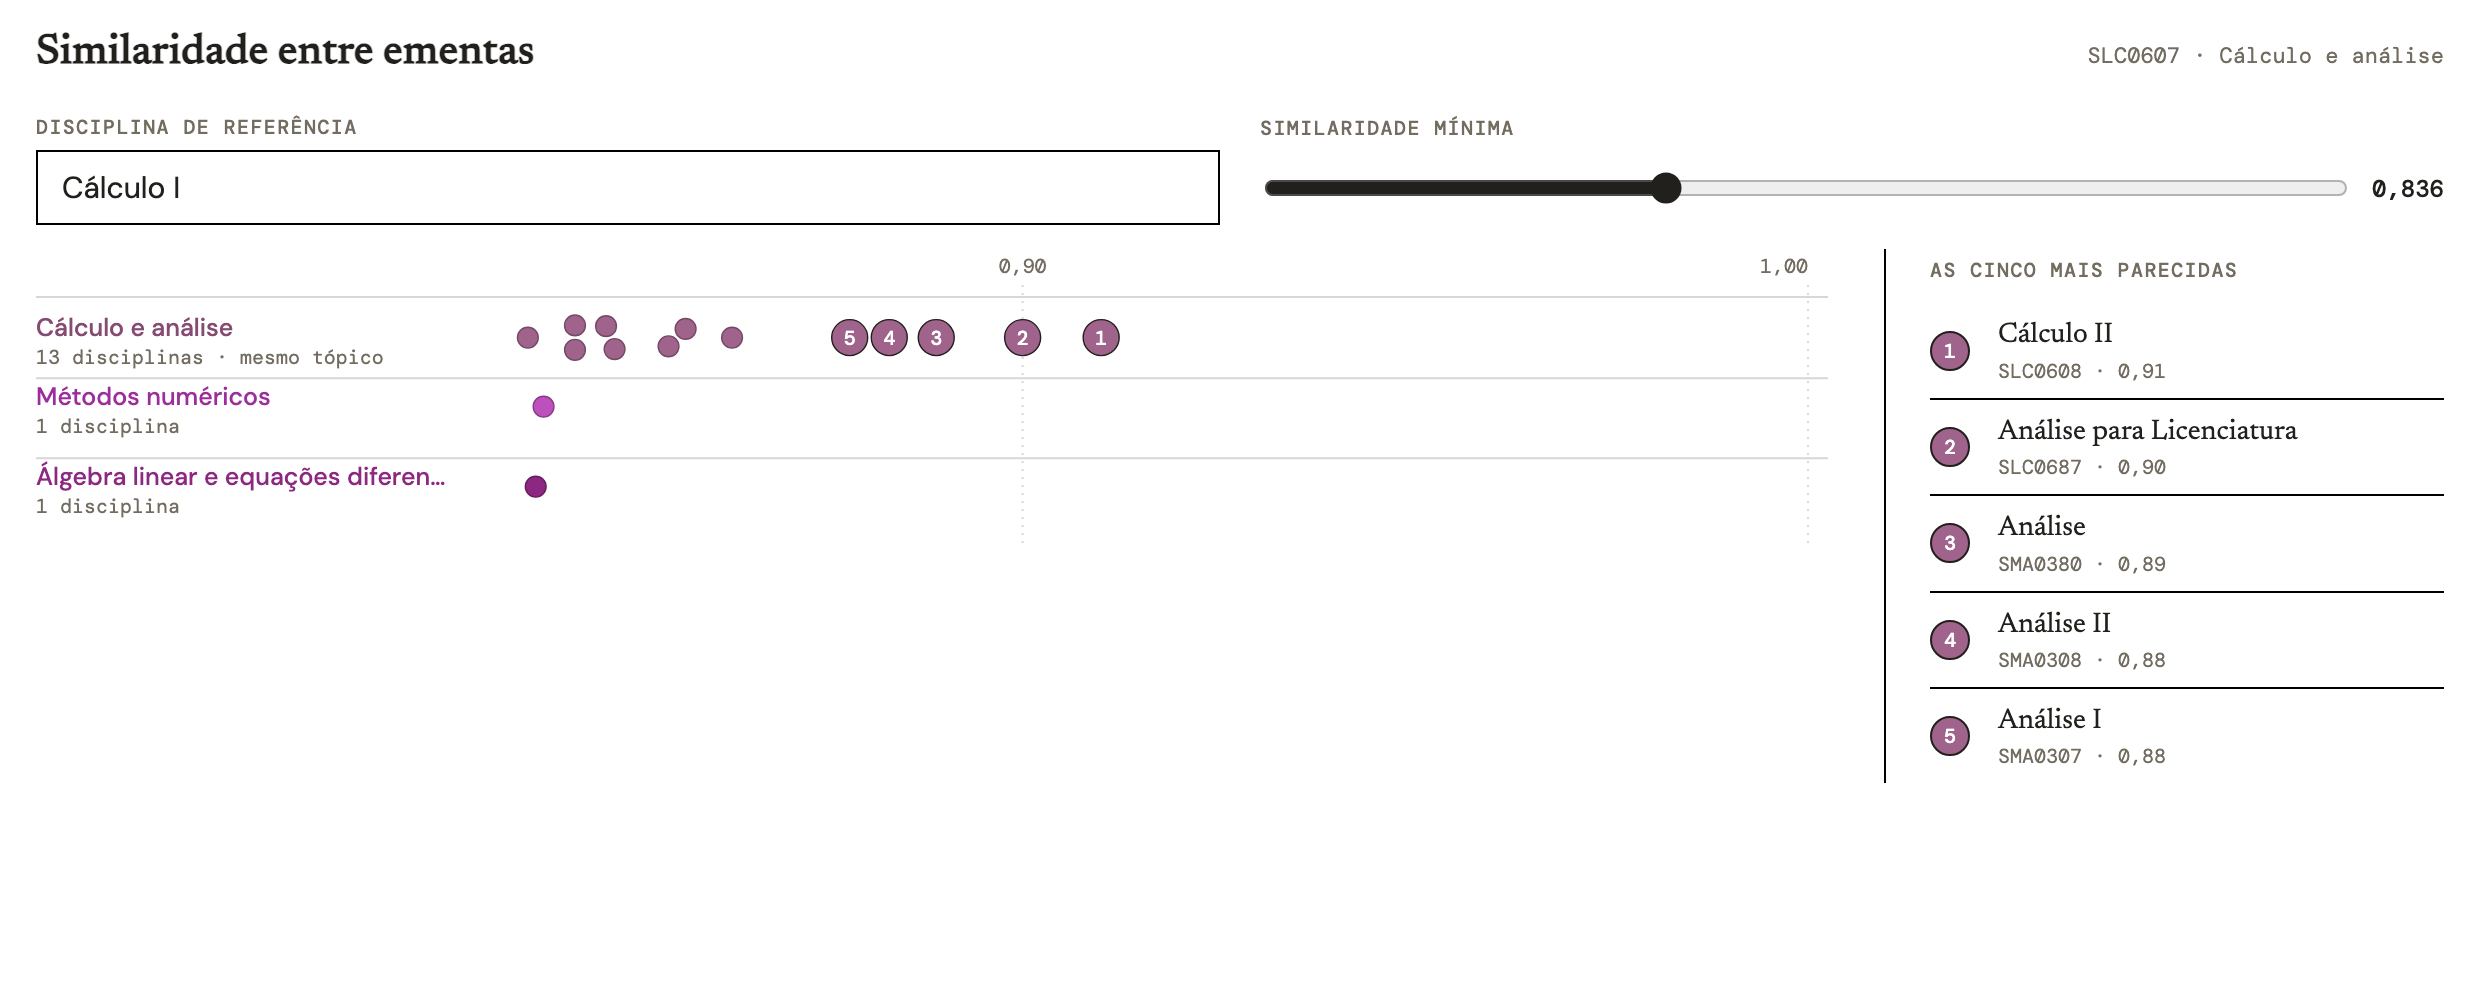
\includegraphics[width=\linewidth]{figures/similaridade.png}
  \caption{Distribuição exibida após selecionar Cálculo I como referência,
  agrupada por tópico. A posição horizontal representa a similaridade de
  cosseno, e o índice identifica as cinco disciplinas mais próximas.}
  \label{fig:similaridade}
\end{figure}

\subsection{Grade e requisitos}

Como requisitos são relações dirigidas que se distribuem ao longo do curso, a
grade dispõe as disciplinas por semestre ideal, de modo que a ordem curricular
fique visível. A Figura~\ref{fig:grade} organiza a grade escolhida em colunas de semestre ideal.
Disciplinas obrigatórias têm preenchimento intenso, e optativas têm
preenchimento claro e contorno tracejado. Ao selecionar uma disciplina, o usuário vê seus
requisitos diretos e indiretos e as disciplinas que ela libera. São consideradas
as relações de requisito e de requisito fraco entre disciplinas da grade.
Indicações de conjunto são excluídas, pois pedem que duas disciplinas sejam
cursadas juntas e não estabelecem precedência. As relações não
são desenhadas permanentemente, pois 897 pares distribuídos por 12 grades
causariam sobreposição.

\begin{figure}[htbp]
  \centering
  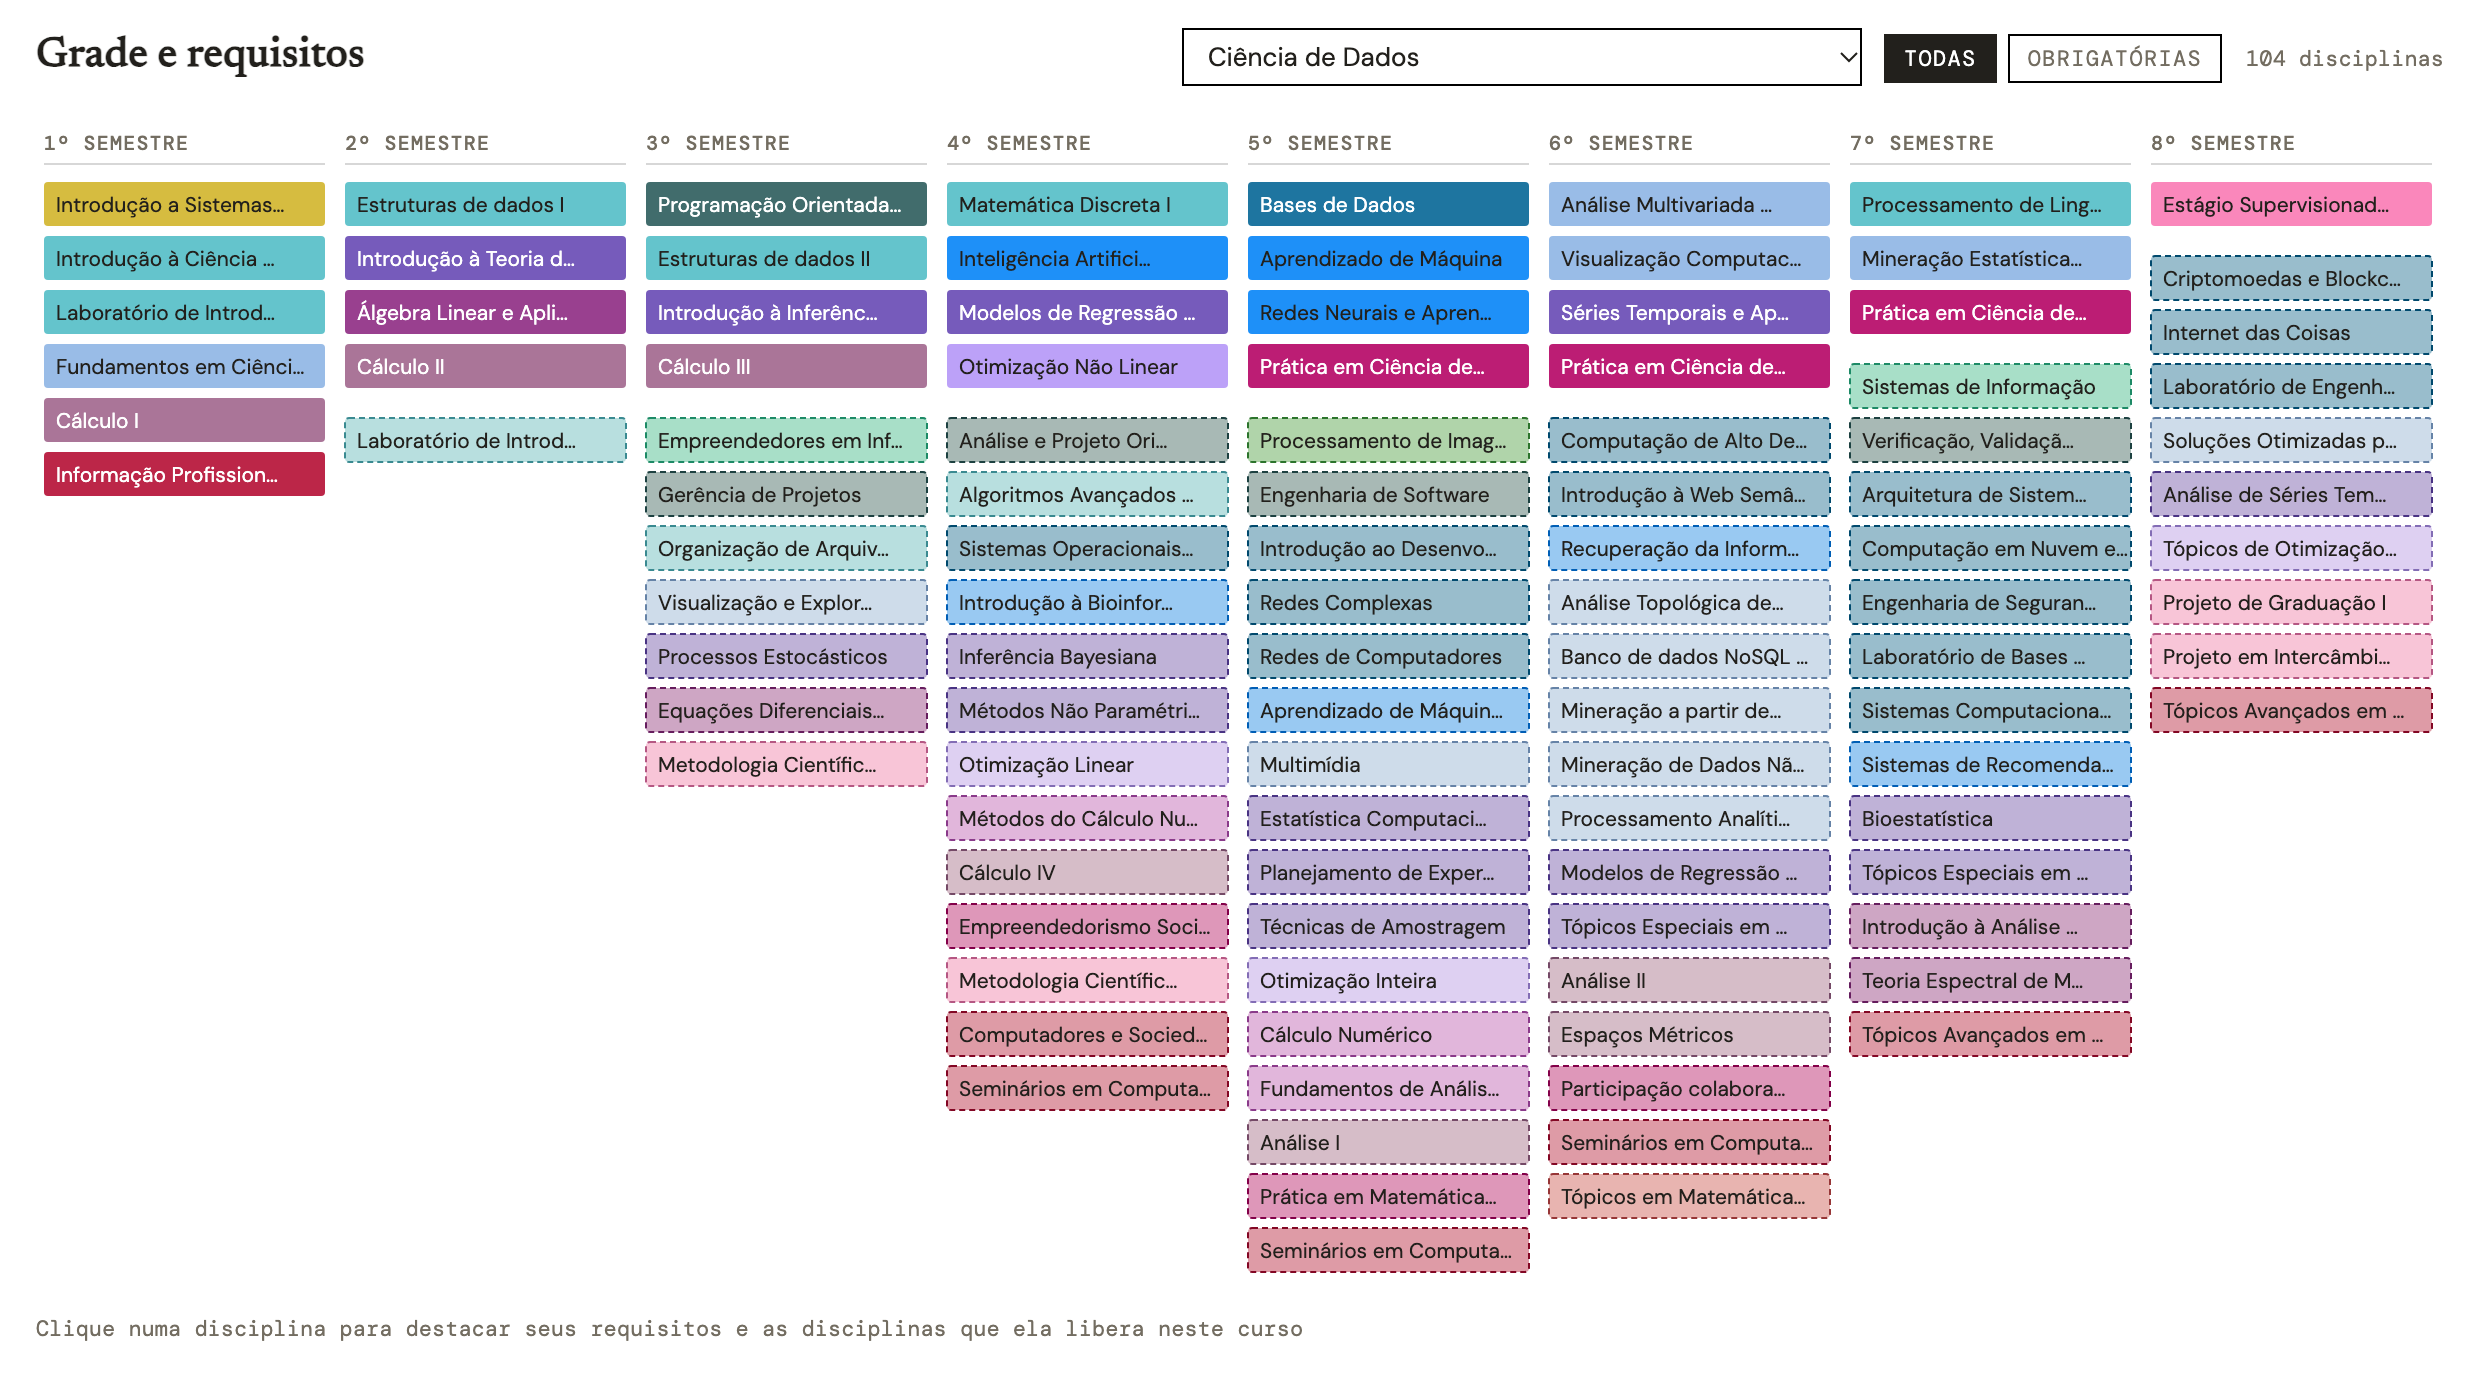
\includegraphics[width=\linewidth]{figures/grade.png}
  \caption{Grade exibida após selecionar Ciência de Dados, antes de destacar
  uma disciplina. As colunas representam os semestres ideais e as cores indicam
  os tópicos das disciplinas.}
  \label{fig:grade}
\end{figure}

\subsection{Composição por tópico}

O treemap organiza as disciplinas da grade escolhida dentro de seus tópicos.
A área de cada retângulo é proporcional à carga horária da disciplina, e a
porcentagem de um tópico usa como denominador a soma das cargas horárias
exibidas. O controle de curso e o filtro de obrigatórias são compartilhados
com a grade, de modo que as duas visões mudam juntas. As disciplinas
obrigatórias têm preenchimento intenso e as optativas, preenchimento claro.
Ao selecionar uma disciplina no treemap, o mapa e a comparação de similaridade
passam a usar a mesma referência. A Figura~\ref{fig:treemap} mostra apenas as
disciplinas obrigatórias de Ciência de Dados.

\begin{figure}[htbp]
  \centering
  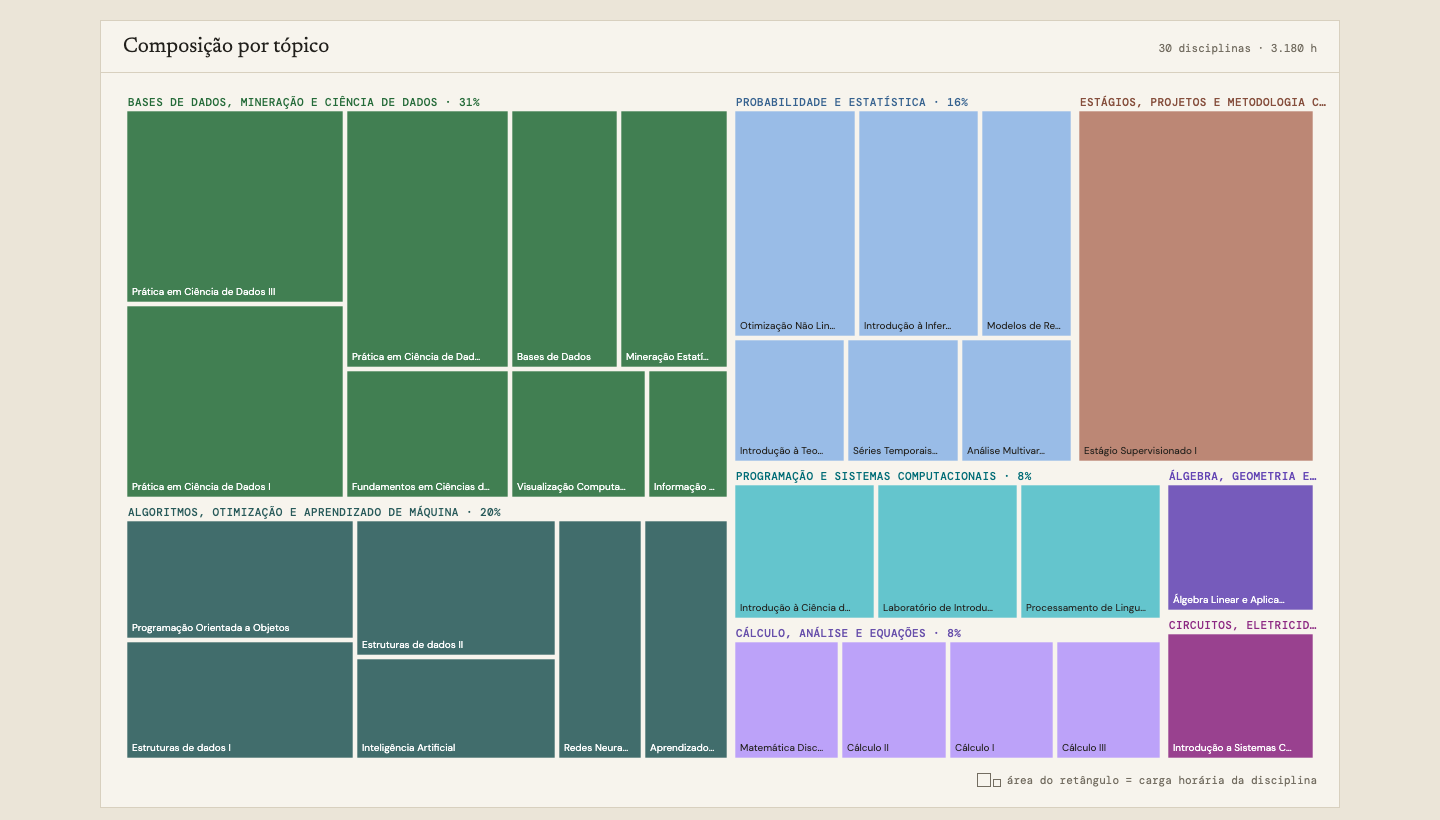
\includegraphics[width=\linewidth]{figures/treemap.png}
  \caption{Composição temática das 30 disciplinas obrigatórias de Ciência de
  Dados com carga horária informada. A área corresponde à carga horária, e as
  porcentagens referem-se às 3.180 horas exibidas.}
  \label{fig:treemap}
\end{figure}

\FloatBarrier

\subsection{Coordenação entre visões}

A seleção de uma disciplina na busca, no mapa, na comparação de similaridade ou
no treemap atualiza a ficha, marca a disciplina no mapa e no treemap e a usa
como referência para a comparação de similaridade. A seleção de um tópico na
nuvem de palavras ou no treemap esmaece os demais tópicos no mapa e na
composição. Esses destaques coordenados permitem voltar do termo característico
ao conjunto de disciplinas e de uma disciplina à sua vizinhança textual. O
limiar ajustável da comparação constitui uma segunda forma de interação: uma
consulta dinâmica que modifica a quantidade e a distribuição dos pontos
enquanto o usuário explora a similaridade.

\section{Resultados e discussão}

Esta seção responde às três questões levantadas na introdução e discute o
alcance de cada resposta.

\subsection{Agrupamento das disciplinas}

Os 24 tópicos têm entre 8 e 37 disciplinas. A associação entre tópico e
departamento, identificado pelo prefixo do código, é moderada, com informação
mútua normalizada de 0,47 e, ajustada ao acaso, de 0,40: o texto recupera parte
da organização departamental, mas não a reproduz. Há tópicos concentrados, como
Probabilidade e estatística, com 30 de 32 disciplinas do SME, e tópicos que
atravessam unidades, como Física, mecânica e termodinâmica, que reúne
disciplinas de dez siglas, entre elas IFSC, SLC, SEM e SEL.

A associação apenas moderada indica que departamentos e tópicos organizam as
disciplinas por critérios diferentes. Os departamentos refletem a estrutura
administrativa e a área dos docentes, enquanto os tópicos refletem o conteúdo
descrito nas ementas. Assim, os tópicos que atravessam unidades evidenciam
conteúdos compartilhados que a organização departamental não mostra, como a
física ensinada pelo IFSC, por departamentos da EESC e pela Licenciatura em
Ciências Exatas. Os tópicos, porém, descrevem o texto das ementas, e não o que é
efetivamente ensinado em sala.

As nuvens ajudam a interpretar os nomes atribuídos aos tópicos. Em
Probabilidade e estatística, \emph{modelos}, \emph{testes} e \emph{regressão}
estão entre os termos de maior peso. Em Bases de dados, mineração e ciência de
dados, destacam-se \emph{dados}, \emph{mineração} e \emph{visualização}. A
leitura conjunta do nome e dos termos permite reconhecer o conteúdo que
motivou a classificação sem depender apenas da posição no mapa.

\subsection{Similaridade entre disciplinas}

Na comparação de similaridade, as cinco disciplinas mais próximas de Cálculo I
pertencem ao mesmo tópico e têm similaridade entre 0,75 e 0,79: Análise I,
Cálculo II, Análise para Licenciatura, Análise e Análise II. A comparação
aproxima ementas de conteúdo comum, e não apenas sequências de mesmo nome.

O mesmo exemplo mostra o limite da medida. Cálculo I supera o limiar com 136
disciplinas de 18 tópicos, pois o vocabulário de funções, limites e derivadas
aparece em ementas de muitas áreas. Além disso, a similaridade mede proximidade
textual, e não equivalência curricular: Cálculo II é a segunda disciplina mais
próxima de Cálculo I, mas depende dela como requisito. A visão indica, portanto,
disciplinas comparáveis, e não substituíveis.

Com o limiar inicial de 0,619, a comparação de Cálculo I reúne 136 disciplinas
de 18 tópicos. Ao elevá-lo a 0,700, restam 12 disciplinas, todas no tópico
Cálculo, análise e equações. Essa mudança mostra que a vizinhança mais próxima
é temática, enquanto a cauda de similaridades menores alcança outras áreas.
O controle torna visível a sensibilidade da resposta ao limiar escolhido.

\subsection{Encadeamentos e composição curricular}

Os 897 pares de requisito têm similaridade mediana de 0,64, acima da mediana da
mesma grade (0,56) e do conjunto (0,54): requisitos tendem a ligar textos
próximos. As cadeias mais longas têm de quatro a sete etapas, e as disciplinas
de maior alcance são Cálculo I, em matemática e estatística, e as introdutórias
de programação, em computação.

Como a comparação com a mesma grade controla a proximidade temática de cada
curso, a diferença não decorre apenas de os pares pertencerem ao mesmo
currículo. Ainda assim, a similaridade não determina os requisitos: disciplinas
introdutórias liberam conteúdos aplicados com vocabulário diferente, e os
requisitos também expressam decisões pedagógicas.

O treemap complementa a leitura dos requisitos com a distribuição da carga
horária entre os tópicos. Entre as disciplinas obrigatórias de Ciência de
Dados, Bases de dados, mineração e ciência de dados reúne 990 das 3.180 horas
exibidas (31,1\%),
seguido por Algoritmos, otimização e aprendizado de máquina, com 630 horas
(19,8\%), e Probabilidade e estatística, com 510 horas (16,0\%). No
Bacharelado em Estatística e Ciência de Dados, a concentração é diferente:
Probabilidade e estatística corresponde a 1.230 das 2.700 horas obrigatórias
(45,6\%), enquanto Bases de dados, mineração e ciência de dados soma 210 horas
(7,8\%). A comparação evidencia ênfases distintas em cursos que compartilham
a expressão \emph{Ciência de Dados} no nome.

Ao incluir todas as optativas ofertadas em Ciência de Dados, os três tópicos
mais extensos passam a ter parcelas próximas: 17,4\% em Algoritmos,
otimização e aprendizado de máquina, 17,1\% em Bases de dados, mineração e
ciência de dados e 17,0\% em Probabilidade e estatística. A oferta optativa
amplia a variedade temática disponível, mas essa soma não representa um
percurso individual, pois cada estudante cursa apenas parte das optativas.

\section{Limitações}

Os resultados dependem do conteúdo do JúpiterWeb e da redação das ementas. Os
limiares de consolidação, os parâmetros do UMAP e do HDBSCAN e os nomes dos
tópicos influenciam os agrupamentos. Além disso, 74 disciplinas (14\%) foram
classificadas como ruído pelo HDBSCAN e atribuídas ao tópico de centroide mais
próximo. Disciplinas homônimas com sobreposição parcial, como Física II do IFSC e
Física 2 da Licenciatura em Ciências Exatas, permanecem unidas.

As nuvens exibem termos característicos segundo c-TF-IDF, e não uma lista de
todos os assuntos ensinados. No treemap, as porcentagens dependem do filtro e
da carga horária informada para cada disciplina; registros sem carga horária
são omitidos. A opção \emph{todas} soma as optativas ofertadas na grade,
inclusive alternativas que um mesmo estudante não cursaria conjuntamente.
Portanto, a área não equivale à carga horária necessária para concluir o curso.

\section{Lições aprendidas}

A preparação dos identificadores mostrou-se a etapa mais decisiva. Sem a
consolidação dos códigos, Cálculo I apareceria seis vezes e distorceria tópicos,
similaridades e requisitos, e uma consolidação apenas pelo nome uniria
disciplinas distintas, como Física III e Física 3.

A escolha do modelo de linguagem também afetou os resultados. Um modelo com
janela de 128 tokens exigiria dividir os textos em blocos, e o BGE-M3 permitiu
representar cada disciplina por inteiro. Como a escala da similaridade muda de
um modelo para outro, os limiares passaram a ser definidos por percentis, e não
por valores fixos.

Por fim, a legibilidade exigiu decisões de projeto em cada visão: a repulsão
entre pontos e a numeração das vizinhas no mapa, a exibição sob demanda dos
requisitos na grade e o uso de rótulos junto às cores. Esses ajustes foram mais
úteis que efeitos de animação para tornar as visualizações interpretáveis.

Na segunda entrega, a coordenação entre as visões mostrou-se útil para
relacionar escalas de análise diferentes. A nuvem permite partir de um termo
característico para localizar o tópico no mapa; o treemap permite partir da
composição de um curso para examinar disciplinas e suas vizinhas textuais. O
limiar ajustável expõe quanto a comparação de similaridade depende do recorte
adotado.

\section{Conclusão}

As cinco visualizações permitem examinar as disciplinas como grupos temáticos,
vizinhanças textuais, sequências de requisitos e parcelas da carga horária das
grades. As novas visões tornam explícitos o vocabulário de cada tópico e a
distribuição temática dos cursos. A seleção coordenada e a consulta dinâmica
ligam essas leituras, sem transformar similaridade textual em equivalência
curricular nem a oferta optativa em carga obrigatória.

\begin{thebibliography}{11}

\bibitem{jupiterweb}
UNIVERSIDADE DE SÃO PAULO. \textbf{JúpiterWeb: Sistema de Gestão Acadêmica da
Pró-Reitoria de Graduação}. Disponível em:
\url{https://uspdigital.usp.br/jupiterweb/}. Acesso em: 7 nov. 2026.

\bibitem{chen2024}
CHEN, J., XIAO, S., ZHANG, P., LUO, K., LIAN, D. e LIU, Z. BGE M3-Embedding:
multi-lingual, multi-functionality, multi-granularity text embeddings through
self-knowledge distillation. \textbf{arXiv preprint arXiv:2402.03216}, 2024.

\bibitem{grootendorst2022}
GROOTENDORST, M. BERTopic: neural topic modeling with a class-based TF-IDF
procedure. \textbf{arXiv preprint arXiv:2203.05794}, 2022.

\bibitem{mcinnes2018}
MCINNES, L., HEALY, J. e MELVILLE, J. UMAP: uniform manifold approximation and
projection for dimension reduction. \textbf{arXiv preprint arXiv:1802.03426},
2018.

\bibitem{mcinnes2017}
MCINNES, L., HEALY, J. e ASTELS, S. hdbscan: hierarchical density based
clustering. \textbf{Journal of Open Source Software}, v. 2, n. 11, p. 205, 2017.

\bibitem{bostock2011}
BOSTOCK, M., OGIEVETSKY, V. e HEER, J. D3: data-driven documents.
\textbf{IEEE Transactions on Visualization and Computer Graphics}, v. 17,
n. 12, p. 2301 a 2309, 2011.

\bibitem{scherer}
SCHERER, C. \textbf{Data Visualization \& Information Design}. Disponível em:
\url{https://www.cedricscherer.com/}. Acesso em: 10 nov. 2026.

\bibitem{holtz}
HOLTZ, Y. \textbf{The D3 Graph Gallery}. Disponível em:
\url{https://d3-graph-gallery.com/}. Acesso em: 10 nov. 2026.

\end{thebibliography}

\end{document}
